\documentclass{beamer}
\usepackage{graphicx}
\usepackage{caption}
%\usepackage{subcaption}
\usepackage{color}
\usepackage{amssymb}
\usepackage{xcolor}
\usepackage{wrapfig}
\usepackage{amsmath}
\usepackage[
backend=bibtex,
sorting=none
]{biblatex}
\addbibresource{bibliography.bib}

\setbeamertemplate{navigation symbols}{}
\usetheme{CambridgeUS}
\usecolortheme{beaver} 

\beamersetuncovermixins{\opaqueness<1>{25}}{\opaqueness<2->{15}}

%\pgfdeclareimage[height=2cm]{i4}{pic/acat.pdf}


%\author[Dzmitry Makatun]{\textbf{Dzmitry~Makatun} \inst{1} $^{,}$ \inst{2}}

\author[Dzmitry Makatun]{\textbf{Dzmitry~Makatun} \inst{1} \inst{3} \and J\'er\^ome~Lauret\inst{2}\\ \and Michal~\v{S}umbera \inst{1} \and Hana~Rudov\'a \inst{4}}
\title[FJFI, CTU]{Distributed Data Processing for High Energy Physics} 
\institute [km]
{ 
  \inst{1}%
  Nuclear Physics Institute, Academy of Sciences, Czech Republic
  \pgfdeclareimage[height=2cm]{i1}{pic/ujf.pdf}   
  \and
  \inst{2}%
  Brookhaven National Laboratory, USA
  \pgfdeclareimage[height=2cm]{i2}{pic/STAR.pdf}
  \and
  \inst{3}
Czech Technical University in Prague, Czech Republic  
\pgfdeclareimage[height=2cm]{i3}{pic/ctu.pdf} 
\and
\inst{4}
Faculty of Informatics, Masaryk University, Czech Republic
\pgfdeclareimage[height=2cm]{i6}{pic/fjfi.pdf}
\pgfdeclareimage[height=2cm]{i8}{pic/doe.pdf}
 
\vspace{-4mm}   
  \pgfuseimage{i1}
  \pgfuseimage{i2}
  \pgfuseimage{i3}
  %\pgfuseimage{i4}
  %\pgfuseimage{i5}
  %\pgfuseimage{i6}
  %\pgfuseimage{i8}

  \vspace{-7mm}
\begin{center}
d.i.makatun@gmail.com
\end{center}
\vspace{-5mm}
  }
\begin{document}
\date{\today} 

\begin{frame}
\titlepage
\end{frame}

\begin{frame}\frametitle{Outline}\tableofcontents
\end{frame}

\section{Introduction}

\begin{frame}\frametitle{Computations in HEP: what do we compute?}
\begin{figure}
\begin{center}
%\vspace{-1 cm}
\includegraphics[ height=0.4\textheight]{pic/rhic.jpg}
\hspace{0.5cm}
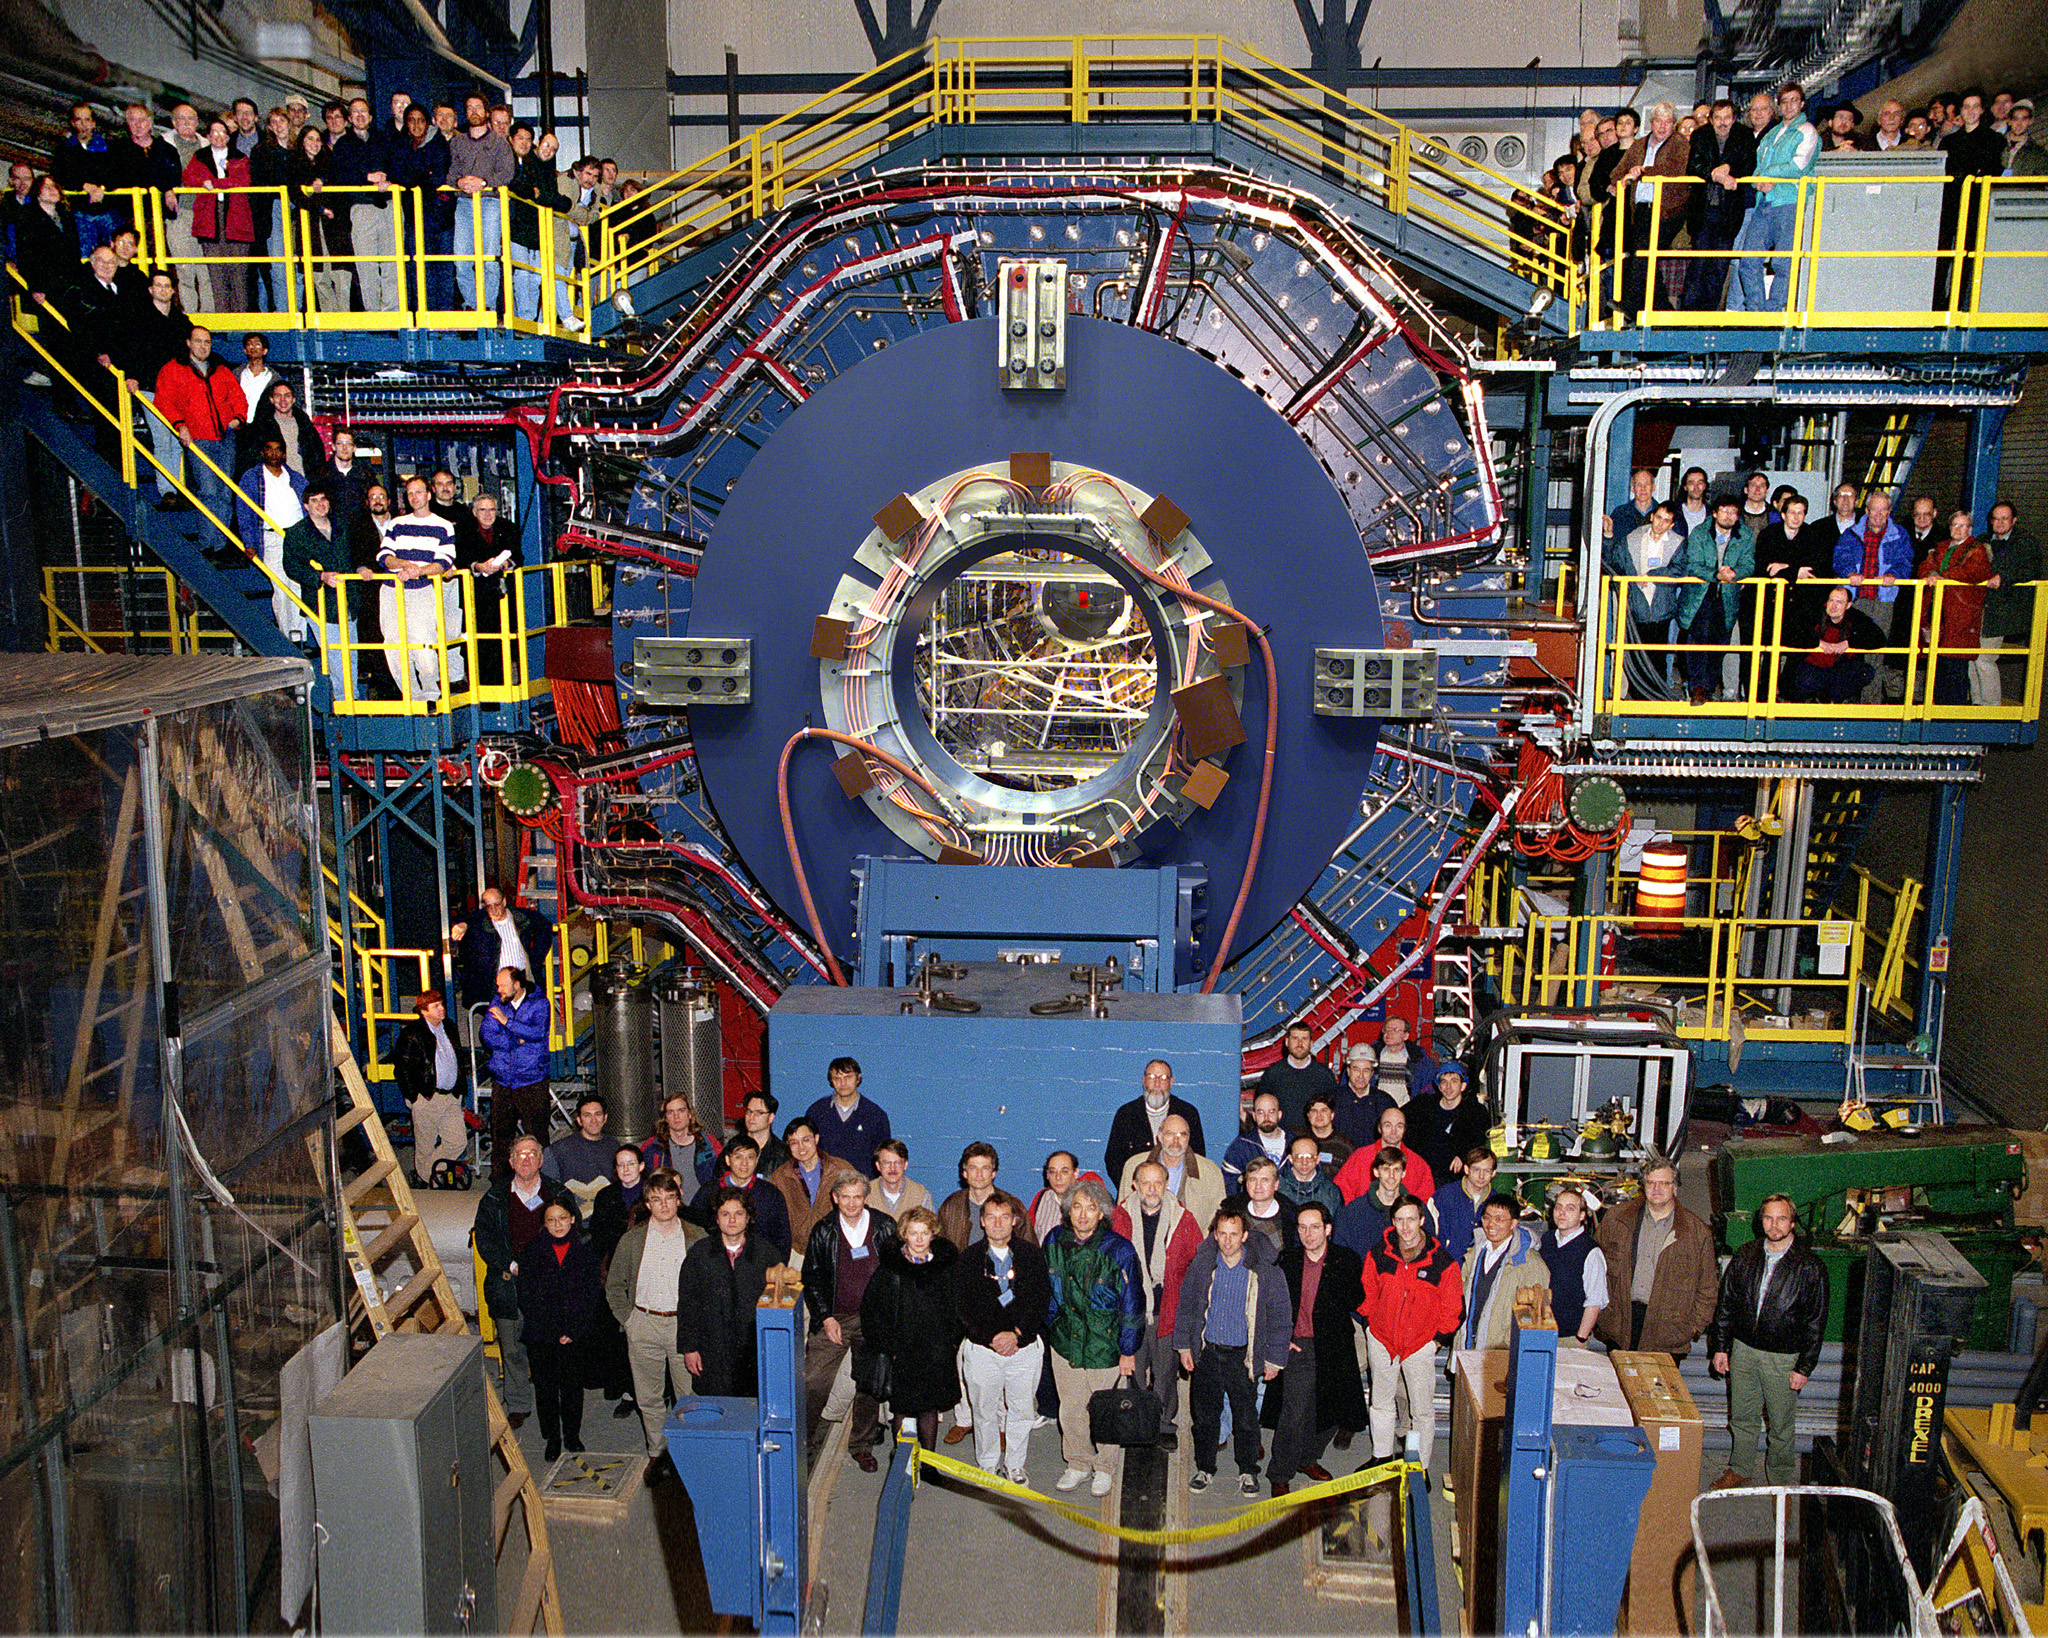
\includegraphics[ height=0.4\textheight]{pic/star.jpg}
\end{center}
\end{figure}
\vspace{-1 cm}
\begin{block}{}
		\begin{itemize}
			\item Brookhaven National Laboratory (\textbf{BNL}) Long Island, NY, USA
			\item Relativistic Heavy Ion Collider (\textbf{RHIC}). In Gold-Gold ion collisions a quark-gluon plasma is created to study the primordial form of matter that existed in the universe shortly after the Big Bang.
			\item Solenoid Tracker at RHIC (\textbf{STAR}). Collisions occur millions of times per second. Events of size 200 MB are processed at input rates up to 100Hz. Output data rate is $\sim$ \textcolor{red} {30 MB/sec}.
		\end{itemize}
 	\end{block}
\end{frame}

\begin{frame}\frametitle{Computations in HEP: how do we compute?}
\begin{block}{}
\textbf{Data Production:} The raw output data is processed to reconstruct events. ($\sim$ ones)\\
\textbf{User Analysis:} Then the reconstructed events are analyzed by scientists to discover new physics. (Each file many times)\\
All the data: raw, reconstructed and analysis output are stored.\\
31 PB of data stored on tape, $\sim$ 12 000 jobs running simultaneously (at RCF only).\\

 	\end{block}
\begin{figure}
\begin{center}
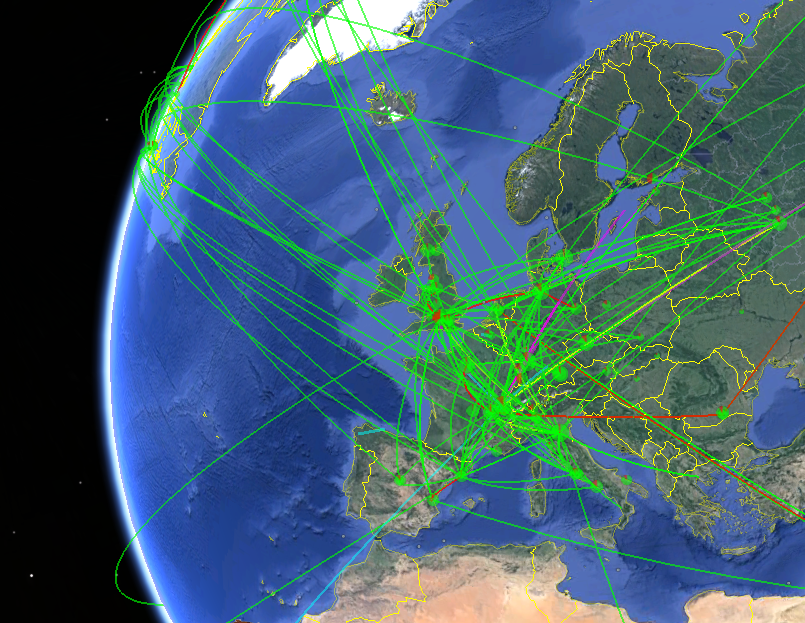
\includegraphics[ height=0.35\textheight]{pic/grid-net.png}
\hspace{0.1cm}
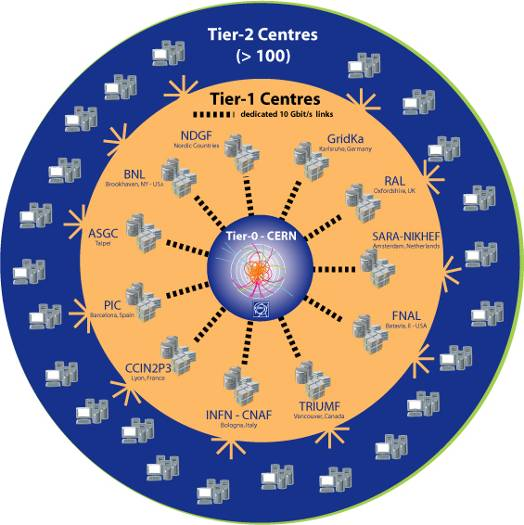
\includegraphics[ height=0.35\textheight]{pic/tiers.jpg}
\hspace{0.1cm}
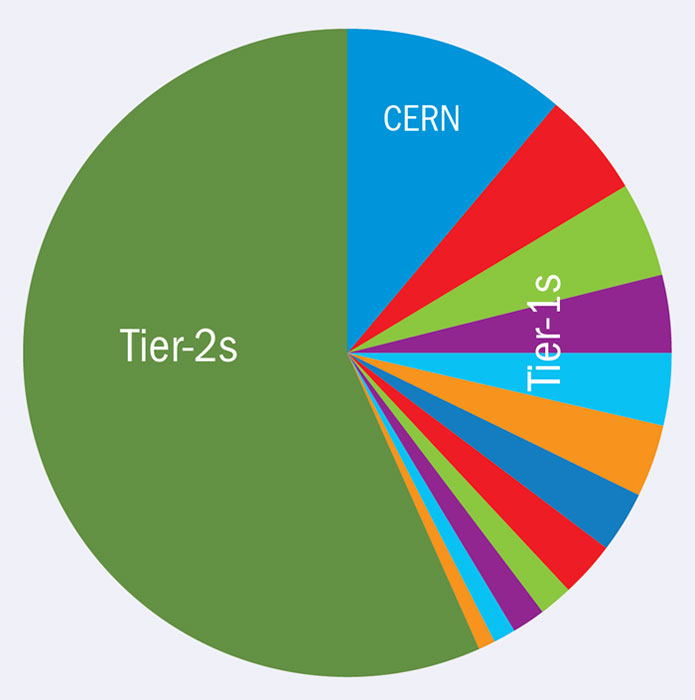
\includegraphics[ height=0.35\textheight]{pic/cern-tier-chart.jpg}
\end{center}
\end{figure} 	
\end{frame}


\subsection{Motivation}
\begin{frame}\frametitle{Previous work and motivation.}
\begin{footnotesize}
\begin{block}{\textbf{RIFT}: \textbf{R}easoner for \textbf{I}ntelligent \textbf{F}ile \textbf{T}ransfer.}
Efficient and controlled movement of replicated datasets within Grid to satisfy multiple requests in the shortest time. \cite{Zerola}
 \begin{itemize}
 % add picture
\item Select between several data sources. 
\item Create optimal transfer paths, merge shared transfer paths of the same file.
\item Schedule transfers on links.
\end{itemize} 
For our class of problems it was shown that global planning of \textbf{data-transferring} over Grid can outperform well known heuristics (e.g. P2P, Xrootd reasoning)
\end{block}  
 		\begin{block}{\textbf{Extension}}
Global planning for jobs coupled with transfers in distributed environment.
 	\end{block} 	
\vspace{-2mm}
\begin{block}{Example of decisions} 
		\begin{itemize}
			\item[?] Send a job to a site with slow connection \textbf{or} wait for a free slot at local site?
		\item[?] Access data remotely \textbf{or} transfer it before the job starts?	
		\end{itemize}
\vspace{-2mm}		
Heuristics such as  \texttt{[Pull a job when CPU slot is free]} will not give the answer.

\end{block}  	 	
\end{footnotesize} 	
\end{frame}


\subsection{Problem analysis}
\begin{frame}\frametitle{Case 1: Data production. Planning remote site usage. }
 	\begin{columns}[c] % the "c" option specifies center vertical alignment
    \column{.6\textwidth} % column designated by a command 	
    \begin{footnotesize}
    \vspace{-11mm}
	\begin{block}{}
		\begin{itemize}
		\item RAW data is located at BNL.
		\item Computational resources are available at BNL and several remote sites.
		\item 1 job per file.
		\item 1 CPU per job. 
		\item Input size $\approx$ Output size
		\item Output file has to be transferred back to BNL.
		\item \textbf{How should we distribute a given set of files between sites to complete the processing faster?}
		\end{itemize}
 	\end{block} 	
 	
 	\begin{block}{}
 	Manually adjust the number of remote jobs to meet the network throughput, \textbf{but} what if:
		\begin{itemize}
		\item[-] More sites
		\item[-] Changing network load
		\end{itemize}
	This should be automated.
 	\end{block} 	
 	     

 	\end{footnotesize}
 	\column{.4\textwidth}
 		\vspace{-5mm}
		\begin{figure}   
				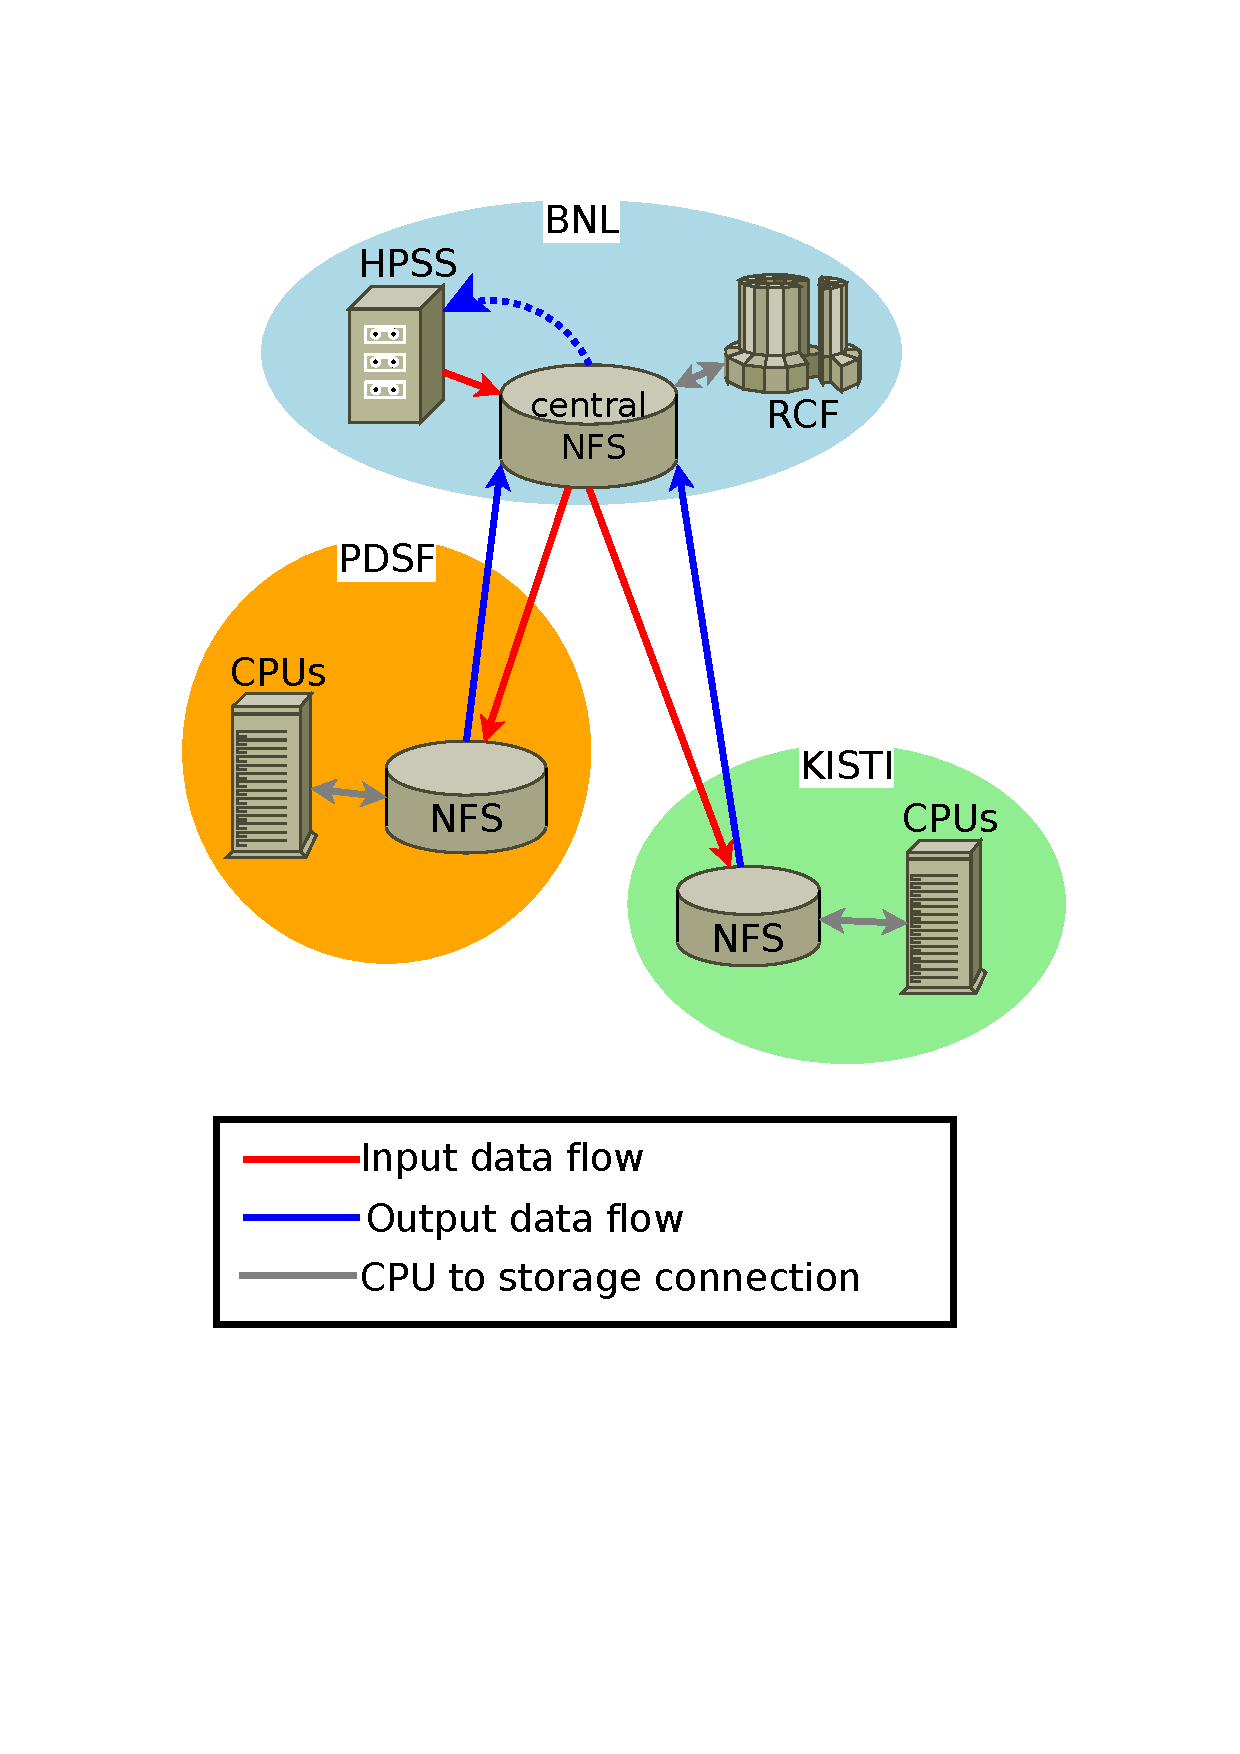
\includegraphics[trim = 25mm 10mm 0mm 30mm, clip, width=1.2\textwidth]{pic/Data_production_schema2.pdf}
		\end{figure} 	 	
 	\end{columns}
\end{frame}


\begin{frame}\frametitle{Case 2: Data production. Optimization. }
 	\begin{columns}[c] % the "c" option specifies center vertical alignment
    \column{.5\textwidth} % column designated by a command 	
    \begin{footnotesize}
    \vspace{-20mm}
	\begin{block}{Consider entire GRID}	
		\begin{itemize}		
			\item Several possible data sources.
			\item More complex network.
			\item Limited storage at sites.
			\item \textbf{How to distribute jobs by sites?}
			\item \textbf{Which file source to select?}
			\item \textbf{What is the optimal transfer path?}

		\end{itemize}
 	\end{block}
		\begin{block}{Example: data-production at ANL  \cite{Balewski}}	
		\begin{itemize}
			\item ANL: many CPU's, but slow connection and small disk space.
			\item NERSC: fast connection, large disk.
			\item Optimization: Feed ANL from both BNL and NERCS sites.		

		\end{itemize}
 	\end{block}
 	\end{footnotesize} 
 	\column{.45\textwidth}
		\begin{figure}
			\begin{center}
			    \vspace{-15mm}
				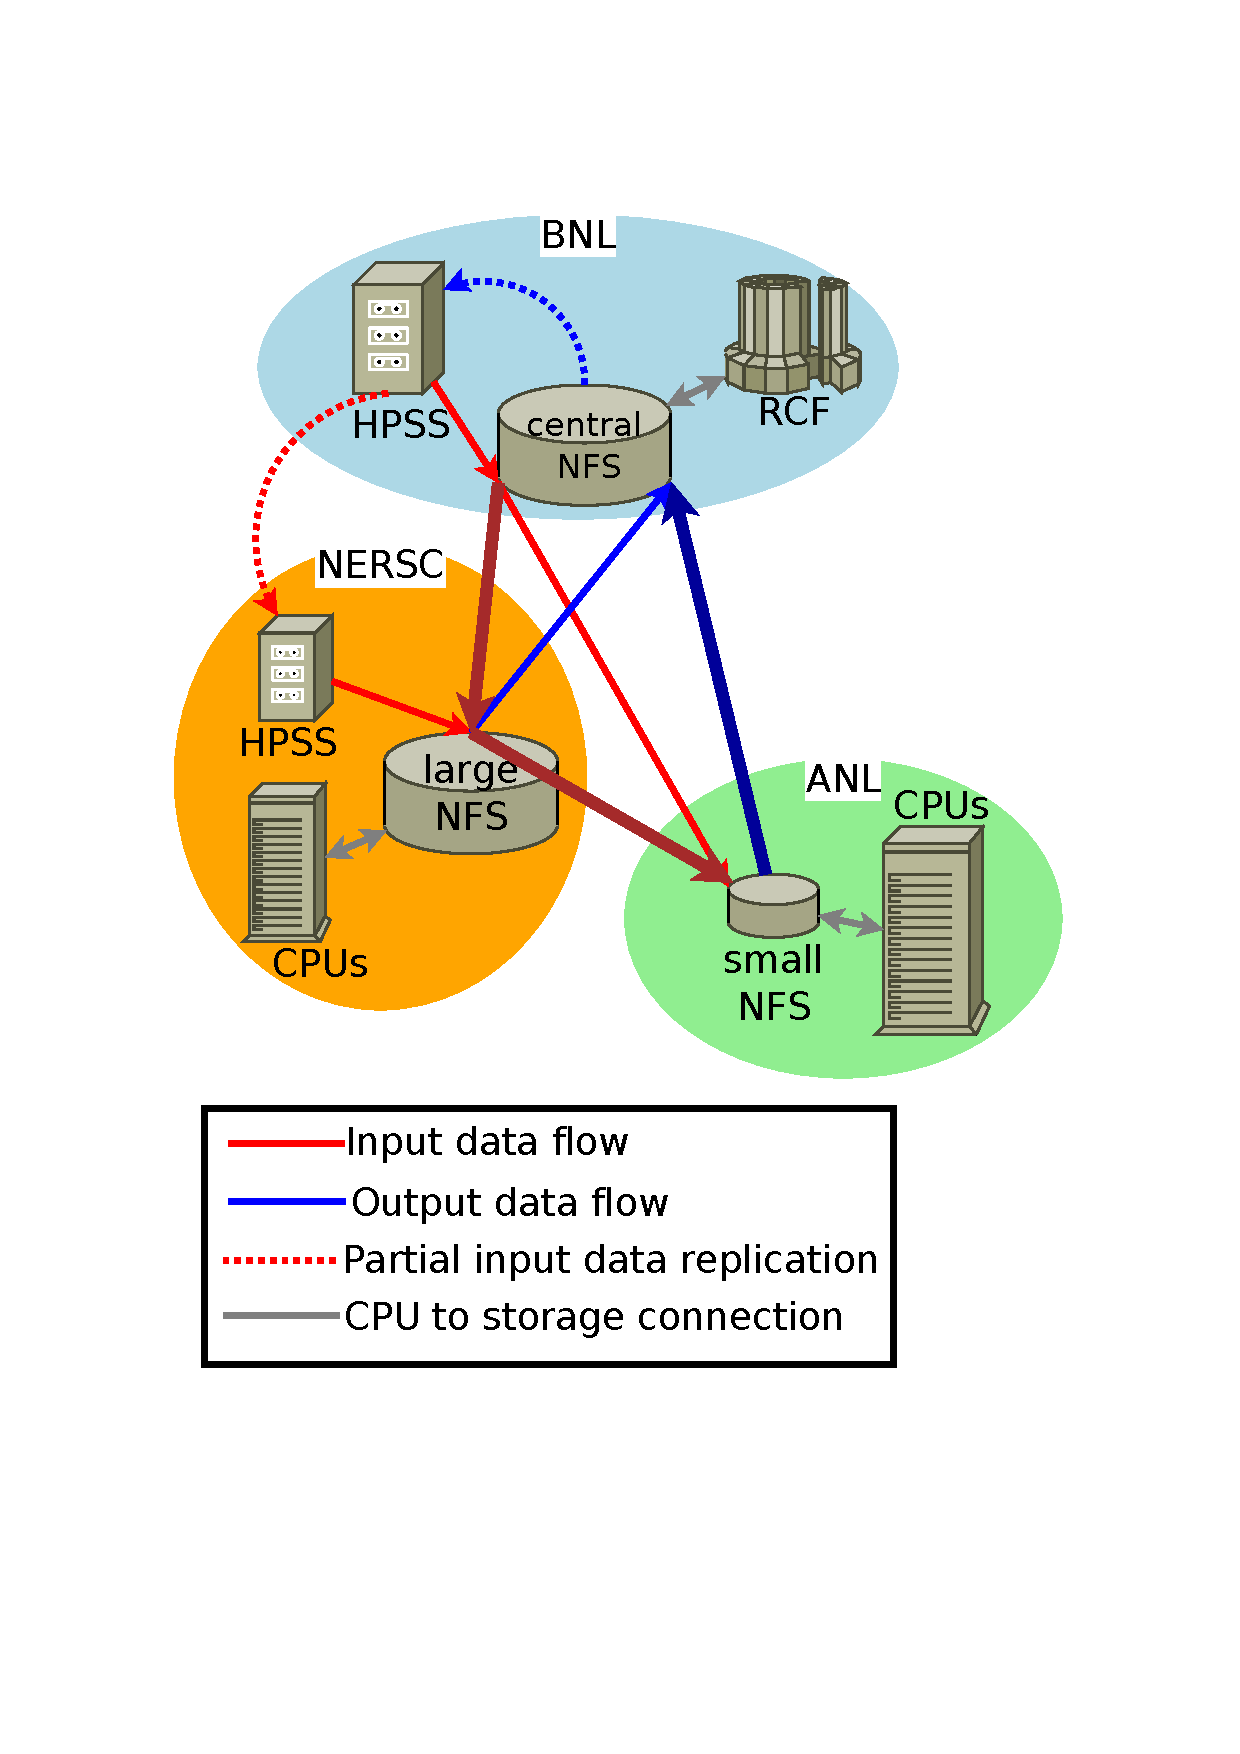
\includegraphics [width=1.2\textwidth]{pic/Data_production_schema_ANL2.pdf}
			\end{center}
			\end{figure} 	 	
 	\end{columns}
\end{frame}


\begin{frame}\frametitle{Case 3: User analysis. }
 	\begin{columns}[c] % the "c" option specifies center vertical alignment
    \column{.5\textwidth} % column designated by a command
 	\begin{small}
 	\vspace{-10mm}
	\begin{block}{}
		\begin{itemize}
			\item Many copies of files exist.	
			\item Each file can be requested by multiple jobs.
			\item 1 CPU per job. 
			\item The size of output of analysis is negligible compared to input size.
			\item The processing time estimates  are imprecise.
			\item \textbf{How to distribute the load?}
			\item \textbf{When and where to replicate the data?}
		\end{itemize}
 	\end{block} 	
 	\end{small}
 	\column{.45\textwidth}

		\begin{figure}
			\begin{center}
			    \vspace{-15mm}
				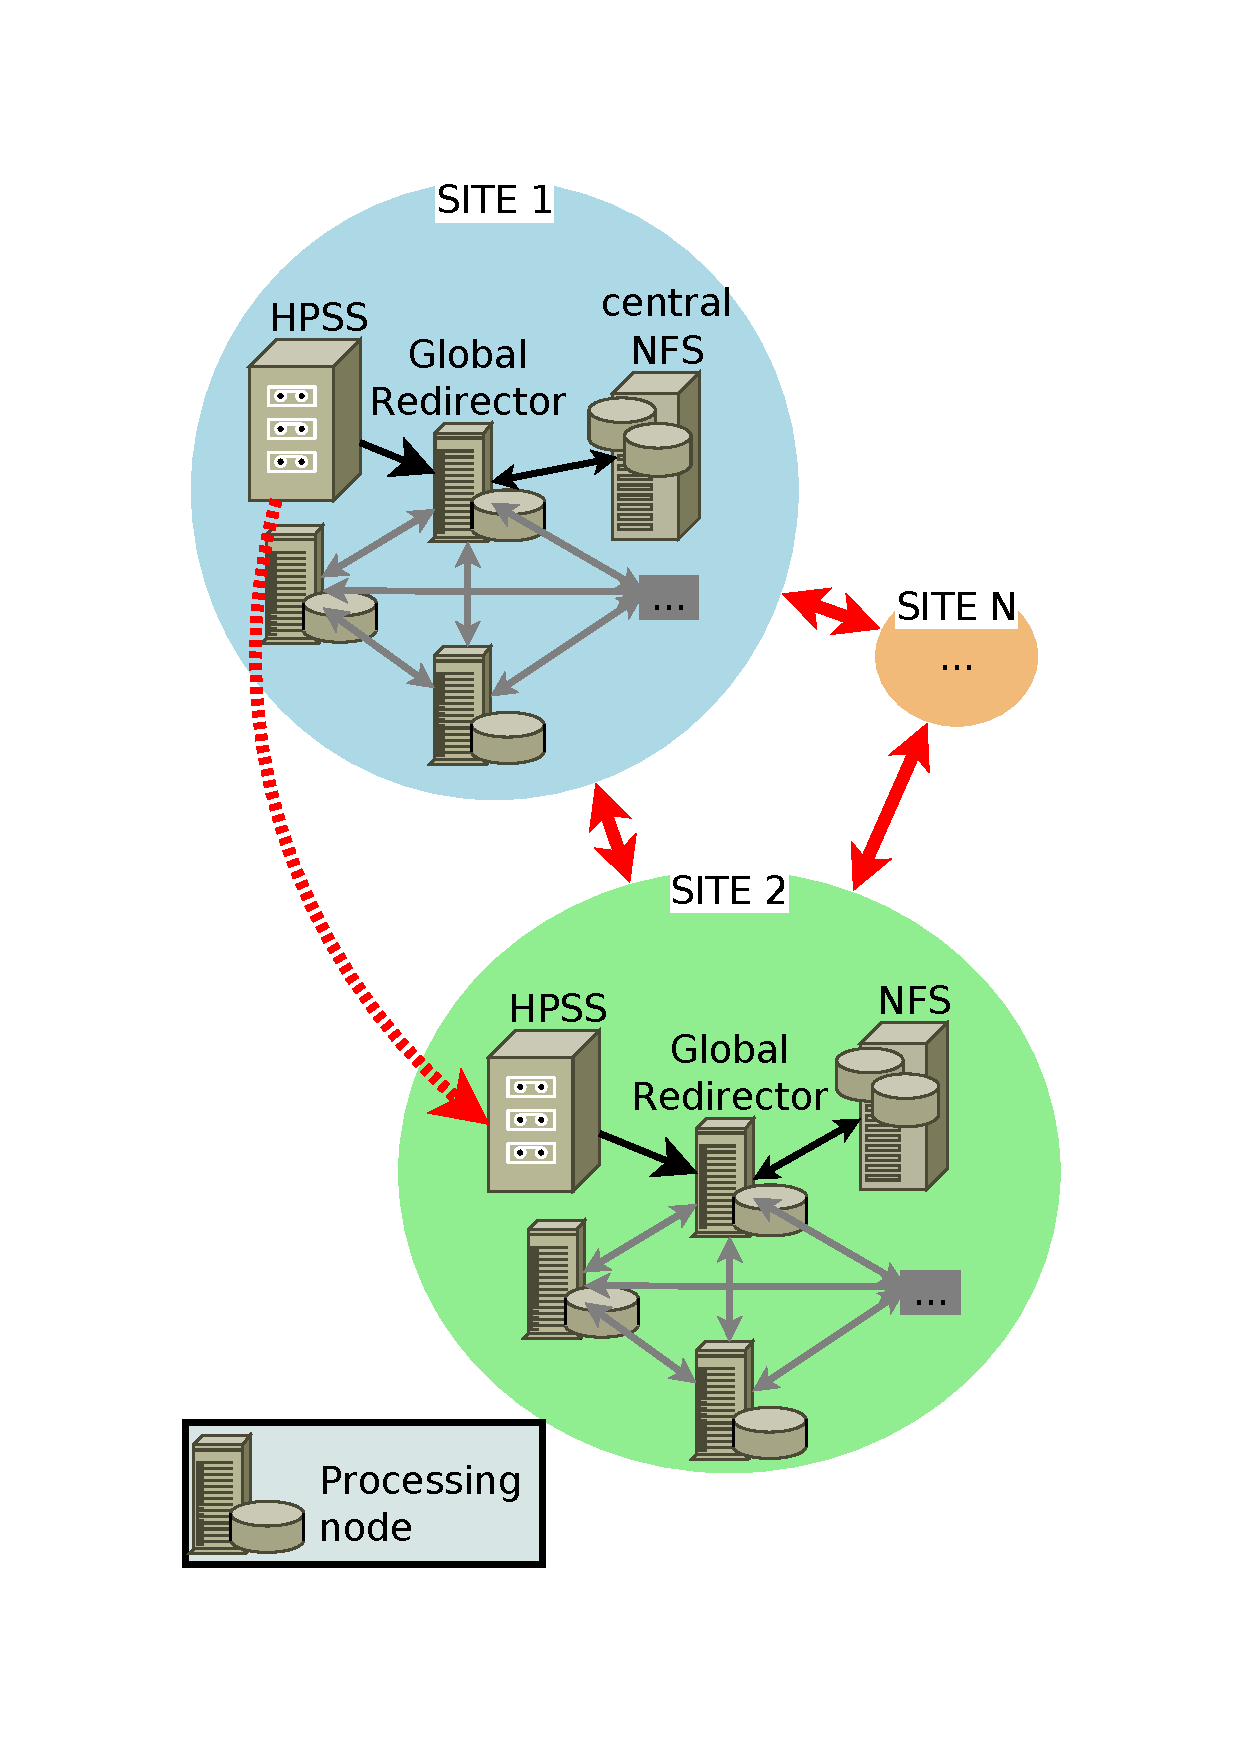
\includegraphics[ width=1.15\textwidth]{pic/user_analysis.pdf}
			\end{center}
			\end{figure} 	 	
 
 	\end{columns}
\end{frame}

\section{Existing solutions}
\begin{frame}\frametitle{STAR: setup for data production at a remote site (KISTI)}
\begin{figure}
\begin{center}
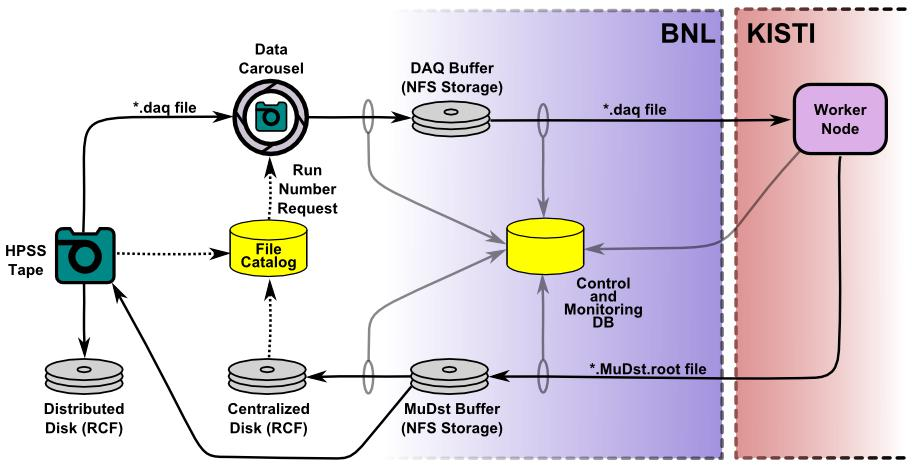
\includegraphics[ width=\textwidth]{pic/kisti_production.jpg}
\end{center}
\end{figure}
\begin{block}{}
		\begin{itemize}
			\item For better efficiency an ad-hock setup is used. \cite{KISTI}
		\end{itemize}
 	\end{block}
\end{frame}




\begin{frame}\frametitle{Existing solutions (simulations)} 	
\begin{footnotesize}
\begin{block}{Bandwidth-Centric Allocation of Independent Tasks on Heterogeneous Platforms \cite{Trees}}  
		\begin{itemize}
			\item Exact solution for maximum steady-state throughput. 
			\item Grid network is modeled as a tree (no alternative paths). Single source/destination. Input path $=$ Output path. Equal size of jobs/files.		
		\end{itemize}
 	\end{block}

\begin{block}{XSufferage \cite{casanova2000heuristics}
}	
\begin{itemize}
 	 \item Considers I/O transfer latency. Assigns jobs to hosts based on $Sufferage = SecondBestEstimatedMakespan - BestEstimatedMakespan$
 	 \item No path/source selection or transfer planning. Simplified network model. No storage model.
 	 \end{itemize}
\end{block}  	
 	
 	
\begin{block}{Storage Affinity \cite{santos2005exploiting}}	
	 \begin{itemize}
	 \item XSufferage + job replication: Executes copies of the same job at several clusters concurrently.
	 \item Simplified network model. CPU waste $\sim 25-60$\%.
 	  \end{itemize}
\end{block}

	 
\end{footnotesize}
\end{frame}


\begin{frame}\frametitle{Existing solutions (in use)} 	
\begin{block}{Batch System + Distributed Data Management System (Independent)}  
		\begin{itemize}
			\item PBS, Condor. [Pull a job from global queue]
			\item Xrootd, DPM. [Site which replies first is selected as a source] 			
		\end{itemize}
 	\end{block} 	
\begin{block}{Data Trains (For user analysis)}	
	 \begin{itemize}
	 \item Group jobs by input data $\longrightarrow$ preplace data $\longrightarrow$ start jobs simultaneously $\longrightarrow$ kill latest x\% of jobs. 
	 \item Train runs periodically. ($\sim$ ones per day)  
 	 \item Controlled by train operators. 
 	  \end{itemize}
\end{block}
\begin{block}{Globus (Decoupling jobs and transfers)} 	
\begin{itemize}
 	 \item Sends jobs to data.  
 	 \item Replicate most "popular" files. Relies on usage history.
 	 \item Where to replicate? When to replicate? No transfer planning.
 	 \end{itemize}
\end{block} 	 
\end{frame}

\begin{frame}\frametitle{Distributed resource management system architecture (Globus example) \cite{Globus_scheduler}}
\begin{block}{}
		\begin{itemize}
			\item  The resource broker is acting as a middle tier 
between a user and the resources by doing resource 
matching and job submission for the user. 

		\end{itemize}
 	\end{block}
 	\begin{figure}
\begin{center}
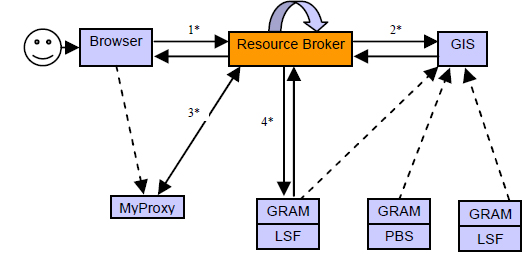
\includegraphics[ width=0.8\textwidth]{pic/resource-broker.jpg}
\end{center}
\end{figure} 	
\end{frame}

\section{Constraint Programming approach}
\subsection{Model}
\begin{frame}\frametitle{Data production problem}
 		\begin{block}{}
Create a global scheduler for Grid which will reason about:\\
\hspace{1cm} 1.data~transferring, \hspace{1cm} 2.~CPU~allocation,\hspace{1cm} 3.~data~storage.  
\end{block}
\begin{block}{Optimization}  
		\begin{itemize}
			\item None of the resources (network links, data storages and CPUs) are over-saturated at any moment of time.
			\item The jobs are executed  where the data is pre-placed.
			\item No excessive transfers or data replication.
			\item Minimal overall makespan for a given set of tasks.
		\end{itemize}
 	\end{block}
\begin{block}{}
\textbf{To solve the problem we applied Constraint programming due to its techniques for scheduling, planning and optimization.}
 	\end{block} 	
\end{frame}

\begin{frame}\frametitle{Data-production problem: Input.}
\vspace{-1cm}
\begin{center}
 	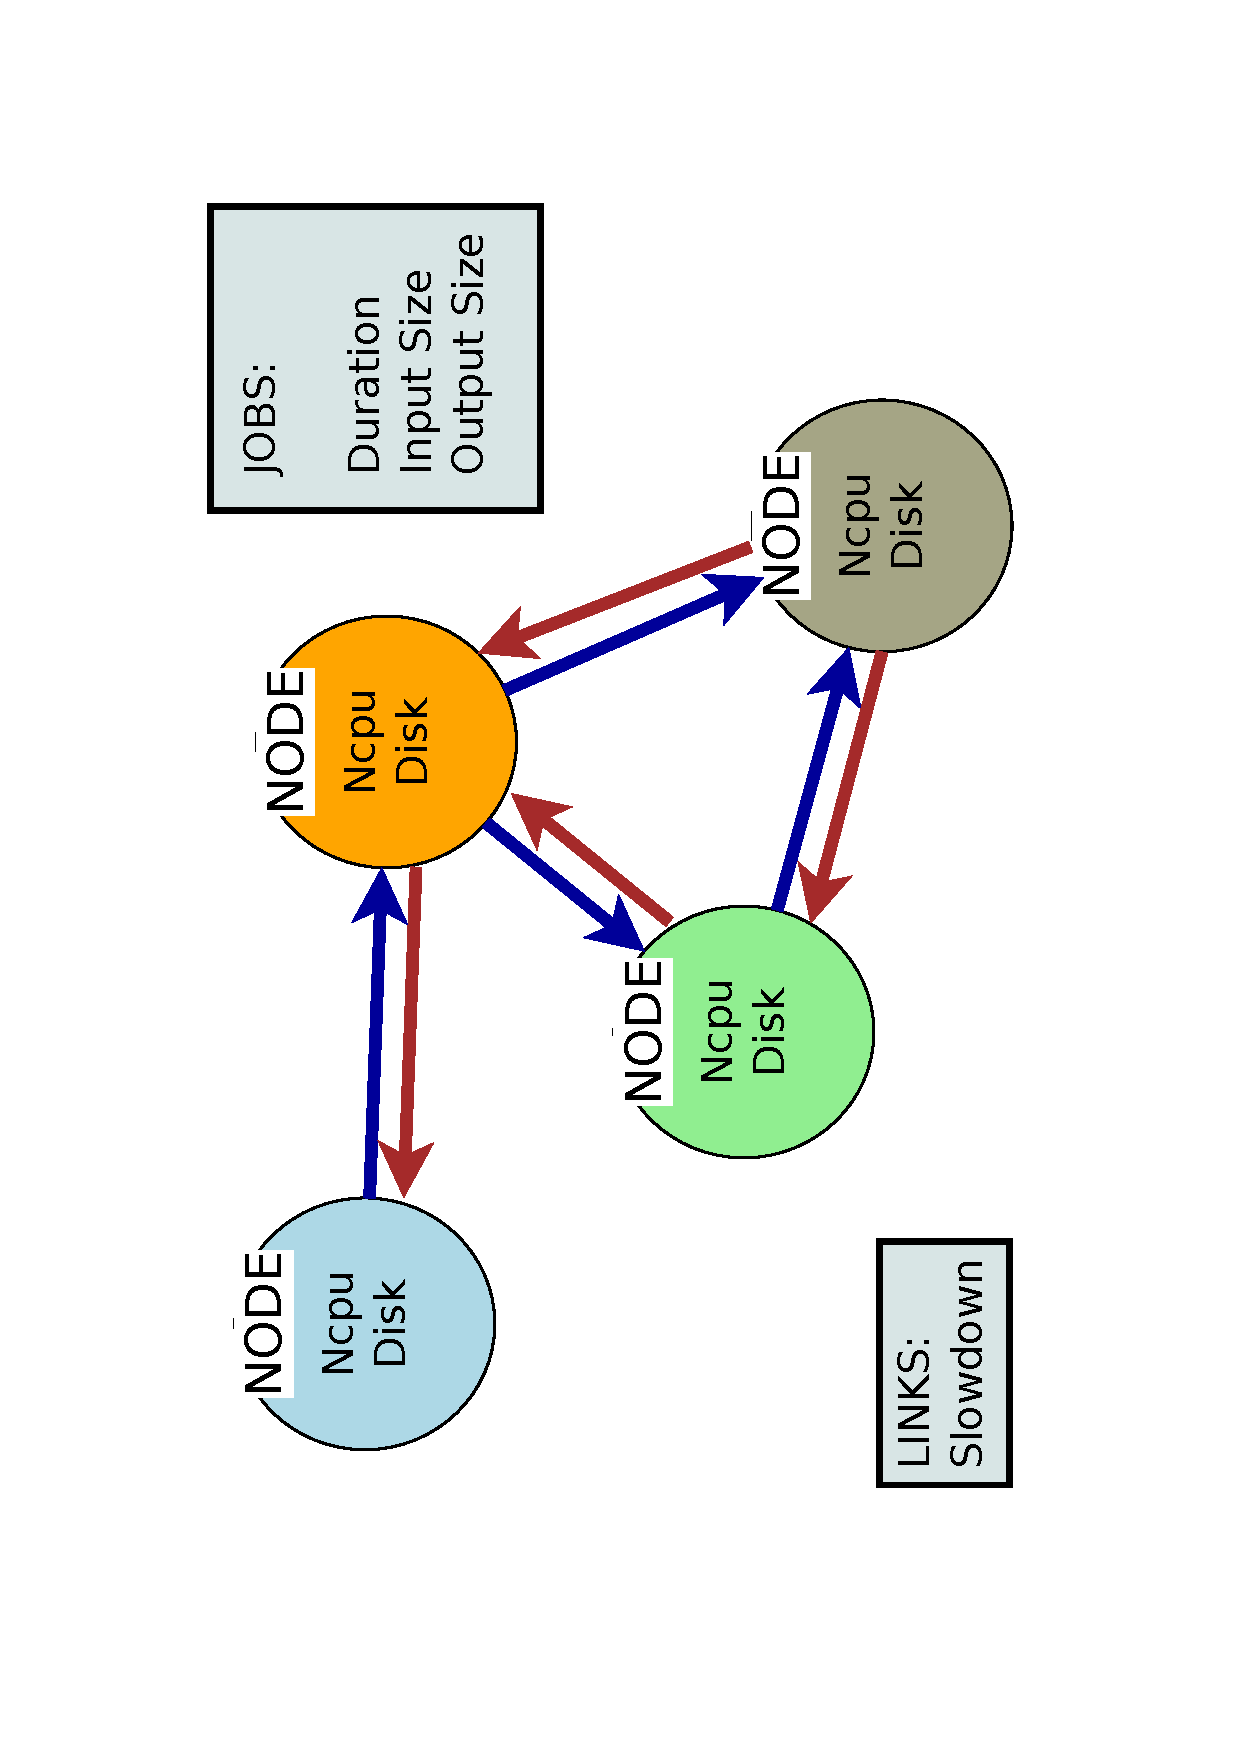
\includegraphics[trim= 30mm 0mm 10mm 0mm,clip,angle =-90, width=0.7\textwidth]{pic/network.pdf}
\end{center}
\vspace{-12mm}
\begin{block}{Assumptions}
In previous work \cite{Zerola} it was proved that:
		\begin{itemize}
			\item There is advantage to plan and schedule jobs by chunks (split the whole set by portions). 
					\begin{itemize}
					\item[+]More adaptability to changing environment.
					\item[+]Faster plan creation.
					\end{itemize}				
			\item The network links can be considered as unary resources: one file-transfer at a time over link.
		\end{itemize}
 	\end{block}
\end{frame}

\begin{frame}\frametitle{Data-production problem: Variables.}
\begin{columns}[c] % the "c" option specifies center vertical alignment
    \column{.5\textwidth} % column designated by a command
\hspace{-4cm}
\begin{block}{Input parameters:}
\begin{itemize}
\item Nodes $c$
\begin{itemize}
\item[-] CPUs: $N_{CPU}(c)$
\item[-] Disk space: $Disk(c)$
\end{itemize}

\item Links $l$
\begin{itemize}
\item[-] Starting Node
\item[-] End node
\item[-] Slowdown = 1 / Bandwidth
\end{itemize}

\item Jobs $j$
\begin{itemize}
\item[-] Duration
\item[-] Input size
\item[-] Output size
\item[-] Input source node(s)
\item[-] Output destination node(s)
\end{itemize}

\end{itemize}
 	\end{block}
 	
\column{.4\textwidth}
\vspace{-4mm}
\begin{block}{Domain variables:}
\begin{itemize}
\item $Y_{jc} \in \{0,1\}$ job j processed at node c. 
\item $X_{fl} \in \{0,1\}$  file $f$ transferred over link $l$.
\item $Js_{j}$ start time of job $j$.
\item $Ts_{fl}$ start time of transfer of file $f$ over link $l$.
\end{itemize}
Dependent on above
\begin{itemize}
\item $Fs_{fc}$ start time of disk space reservation for file $f$ at node $c$.
\item $Fdur_{fc}$ duration of space reservation for file $f$ at node $c$.
\end{itemize}
 	\end{block}
\end{columns} 	

\end{frame}


\begin{frame}\frametitle{Solving procedure overview.}

\begin{enumerate}
\item \textbf{Initialization Stage}. Estimate $TimeLimit$.
\item \textbf{Planning Stage}. Instantiate a part of domain variables with the help of simplified constraints.     
	\begin{enumerate}[a.]
	\item Assign jobs to computational nodes. 
	\item Select transfer paths for input and output files. 
	\item Additional constraints: load balance, etc.
	\item Find a solution for the sub-problem.
	\end{enumerate}
\item \textbf{Scheduling stage}: define start time for each operation. 
	\begin{enumerate} [a.]
	\item Constraints on order of operations. 
	\item Cumulative constraints.
	\item Minimize target function: (e.g. makespan).
	\end{enumerate}
\end{enumerate}
\end{frame}


\begin{frame}\frametitle{Planning stage (core constraints)}
\vspace{-5mm}
		\begin{block}{Each job processed exactly at one node: (job $j$, node $c$)}
	 	
		\begin{center}
					$\forall j \in J: \sum \limits_{c \in C} Y_{jc} = 1$ 	
		\end{center}	
	
		\end{block}
	\begin{block}{Target function $T_{est}$  - estimated makespan.  }
	For each node $c$:
	$T_{Processing} + T_{InputTransfer} + T_{OutputTransfer} \leq T_{est}$
	\end{block}
	
	\begin{block}{Path selection}
\begin{columns}[c] % the "c" option specifies center vertical alignment
    \column{.8\textwidth} % column designated by a command
File can be transferred from/to each node at most once.
\begin{enumerate}[1.]
		\item Transfer input file from sources over 1 link.
		\item Transfer output to final destination over 1 link.
		\item Intermediate node: If $\exists$ incoming transfer $\Leftrightarrow \exists$ outgoing transfer. 
		\item Selected processing node: 1 incoming input transfer, 1 outgoing input transfer.	
		\end{enumerate}
	\column{.2\textwidth}	
	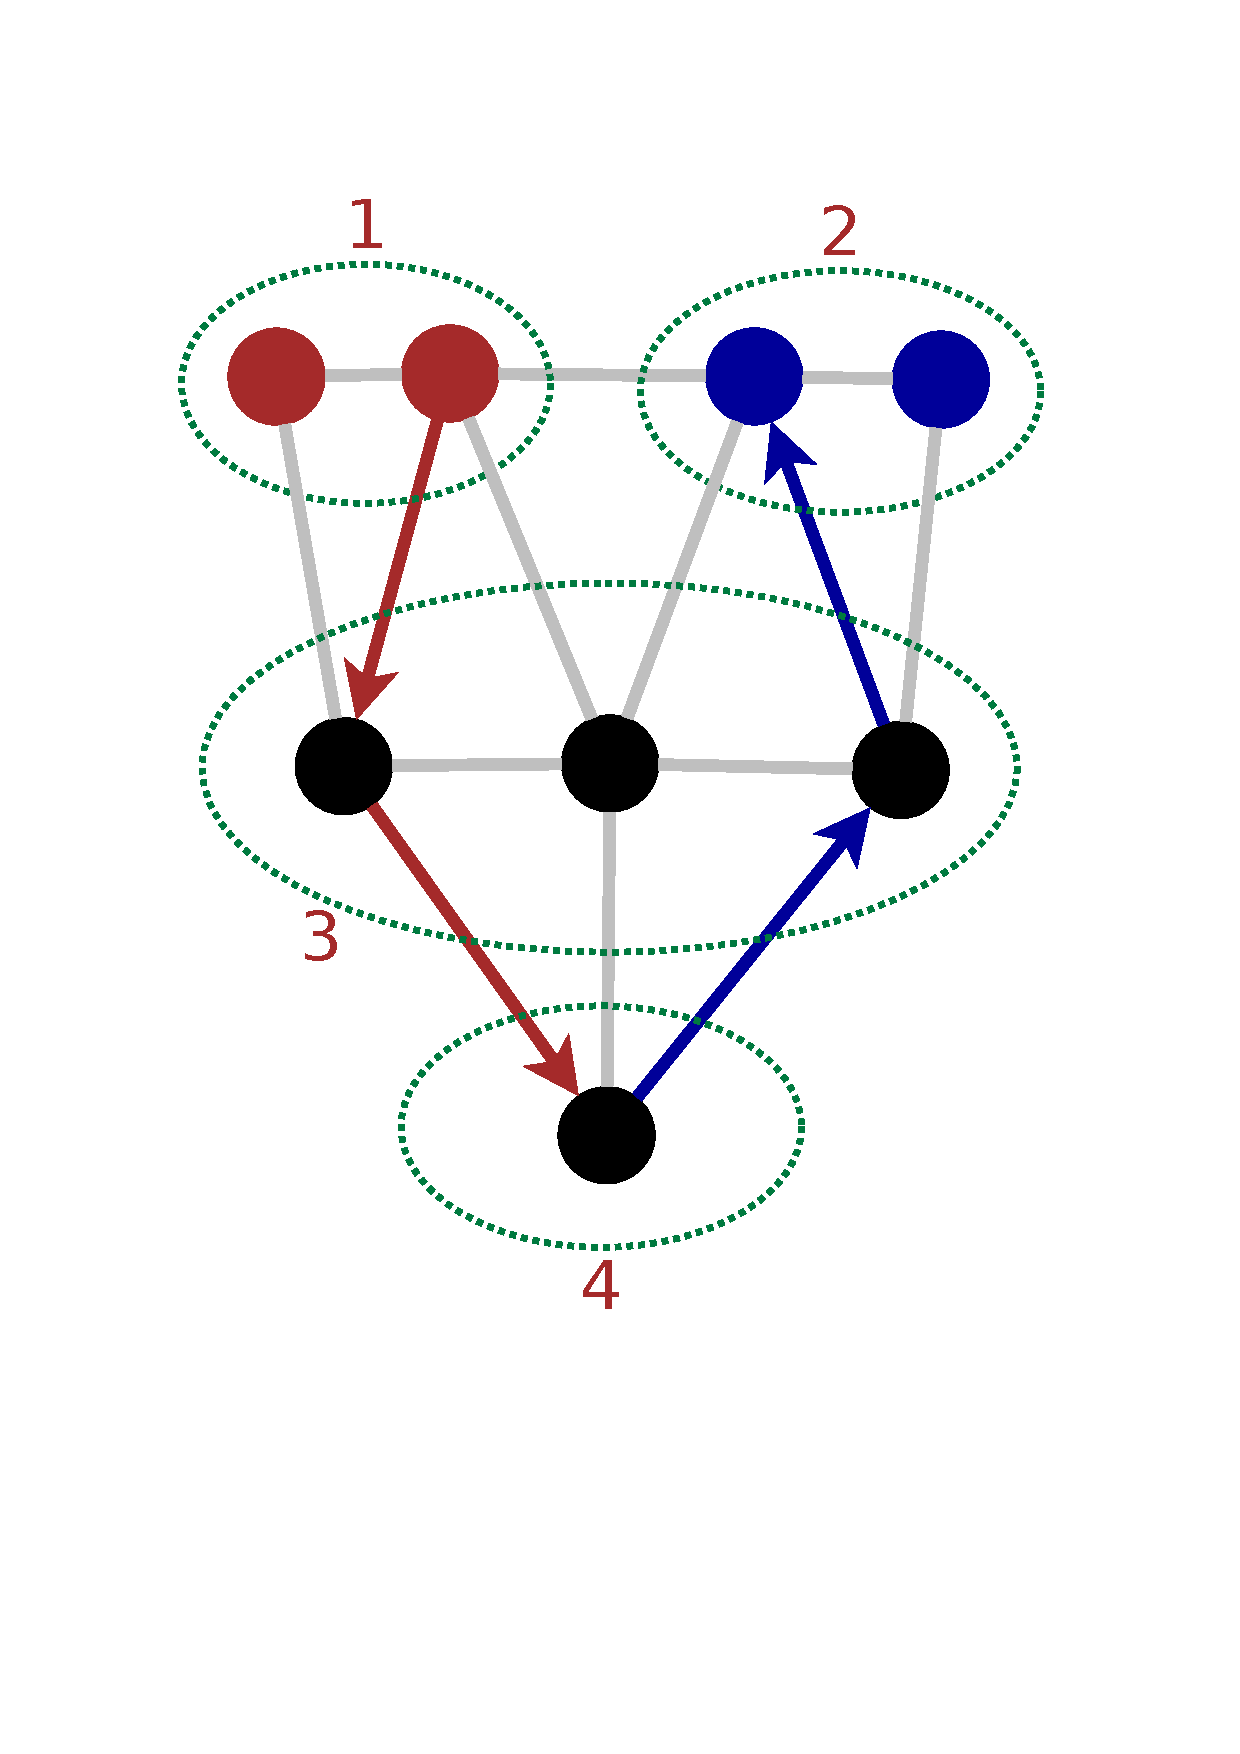
\includegraphics [trim =30mm 70mm 30mm 30mm ,clip, width=\textwidth]{pic/link_selection.pdf}	
	\end{columns}
\end{block}
\end{frame}


		

\begin{frame}\frametitle{Scheduling Stage: order of tasks.}
\begin{block}{Outgoing transfer starts after the incomming one is finished:}
$Ts_{fl}$  transfer start of file $f$ over a link $l$, $c$ is a node. $\forall f \in F, \forall c \in IntermediateNode$:
$$Ts_{fl_{out}} \geq Ts_{fl_{in}} + Size(f) \cdot Slowdown(l_{in}) $$
\end{block}

\begin{block}{Jobs starts after the input file transfer is finished}
$Js_{j}$ start time of a job $j$. $\forall j \in J, l \in L, f = InputFile(j)$
$$Js_{j} \geq Ts_{fl} + Size(f)\cdot Slowdown(l)$$
\end{block}

\begin{block}{Output file is transferred after the job is finished}
$Dur(j)$ is duration of a job $j$.  $\forall j \in J, l \in L, f = OutputFile(j)$
$$Js_{j} +Dur(j) \leq Ts_{fl}$$
\end{block}
\end{frame}

\begin{frame}\frametitle{Scheduling Stage: data placement}
\begin{block}{Space reservation at destination node is made when transfer starts}
$Fs_{fc}$ - start of reservation for file $f$ at node $c$, $Ts_{fl}$  transfer start of file $f$ over a link $l$ to node $c$: \hspace{5mm} $Fs_{fc}=Ts_{fl}$ 

\end{block}
\begin{block}{File can be deleted from start node of a link after the transfer}
$Fdur_{fc}$- duration of file $f$ placement at node $c$, $l$ is outgoing link from $c$
\\ \hspace{30mm}$Fs_{fc}+Fdur_{fc}= Ts_{fl}+Size(f)\cdot Slowdown(l)$
\end{block}

\begin{block}{At selected processing node $c$}
When a job $j$ starts ($Js_j$) then space for output is reserved
$f = OutputFile(j):$ 
 \hspace{20mm}$Fs_{fc}=Js_{j} $
\\When a job finishes its input file can be deleted
$f = InputFile(j):$\\ \hspace{40mm} $Fs_{fc}+Fdur_{fc}=Js_j+Duration(j)  $
\end{block}
\end{frame}


\begin{frame}\frametitle{Scheduling Stage: cumulative constraints.}
\begin{columns}[c] % the "c" option specifies center vertical alignment
    \column{.45\textwidth} % column designated by a command
\begin{block}{cumulative}
Requires that a set of tasks given by \textbf{start times} s, \textbf{durations} d, and \textbf{resource usage} r, never require more than a \textbf{resource limit} b at any time.
\end{block}
\column{.45\textwidth}
\vspace{12mm}
		\begin{figure}
			\begin{center}
			    \vspace{-15mm}
				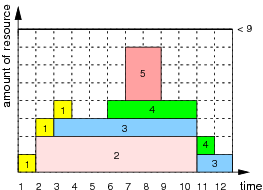
\includegraphics[ scale = .6]{pic/cumulative1.png}
			\end{center}
			\end{figure} 	 	

\end{columns}    
%add picture

\begin{block}{}
\begin{table}\begin{tabular}{ | l | c | c | c | c |   }
  \hline                    
  Task & Start & Duration & Usage & Limit \\ \hline 
  Job & \textcolor{red}{$Js_{jc}$} & $Duration(j)$ & $1$ & $N_{CPU}$(c) \\ \hline
  Transfer & \textcolor{red}{$Ts_{fl}$} & $Size(f)\cdot Slowdown(l)$ & $1$ & 1 \\ \hline
  File placement & \textcolor{red}{$Fs_{fc}$} & \textcolor{red}{$Fdur_{fc}$} & $Size(f)$ & $Disk(c)$ \\ \hline
   
\end{tabular}
\end{table}
\end{block}

\end{frame}

\subsection{Testing simulations}

\begin{frame}\frametitle{Simulations based on log data: problem setup.}
\begin{columns}[c] % the "c" option specifies center vertical alignment
    \column{.6\textwidth} % column designated by a command 	
    \begin{small}
\vspace{-5mm}
 		\begin{block}{Input for simulations}
		\begin{itemize}
			\item Parameters of 2000 jobs taken from log files of data production for STAR at KISTI.
			\item Jobs scheduled by chunks of 200.
			\item Slowdown of the link to the remote site proportional to the \textbf{slowdown factor}.
			\item Makespan compared to local processing.
		\end{itemize}
 	\end{block}
 		\begin{block}{Tested algorithms}
		\begin{itemize}
			\item Equal CPU load.\\ Processed by input order.
			\item Data transferred by job. \\ Processed by input order.
			\item Optimized.\\ Planner: minimize estimated makespan. Scheduler: minimize makespan.
		\end{itemize}
 	\end{block}
 	\end{small} 
 	\column{.4\textwidth}

		\begin{figure}
			\begin{center}
			    \vspace{-20mm}
				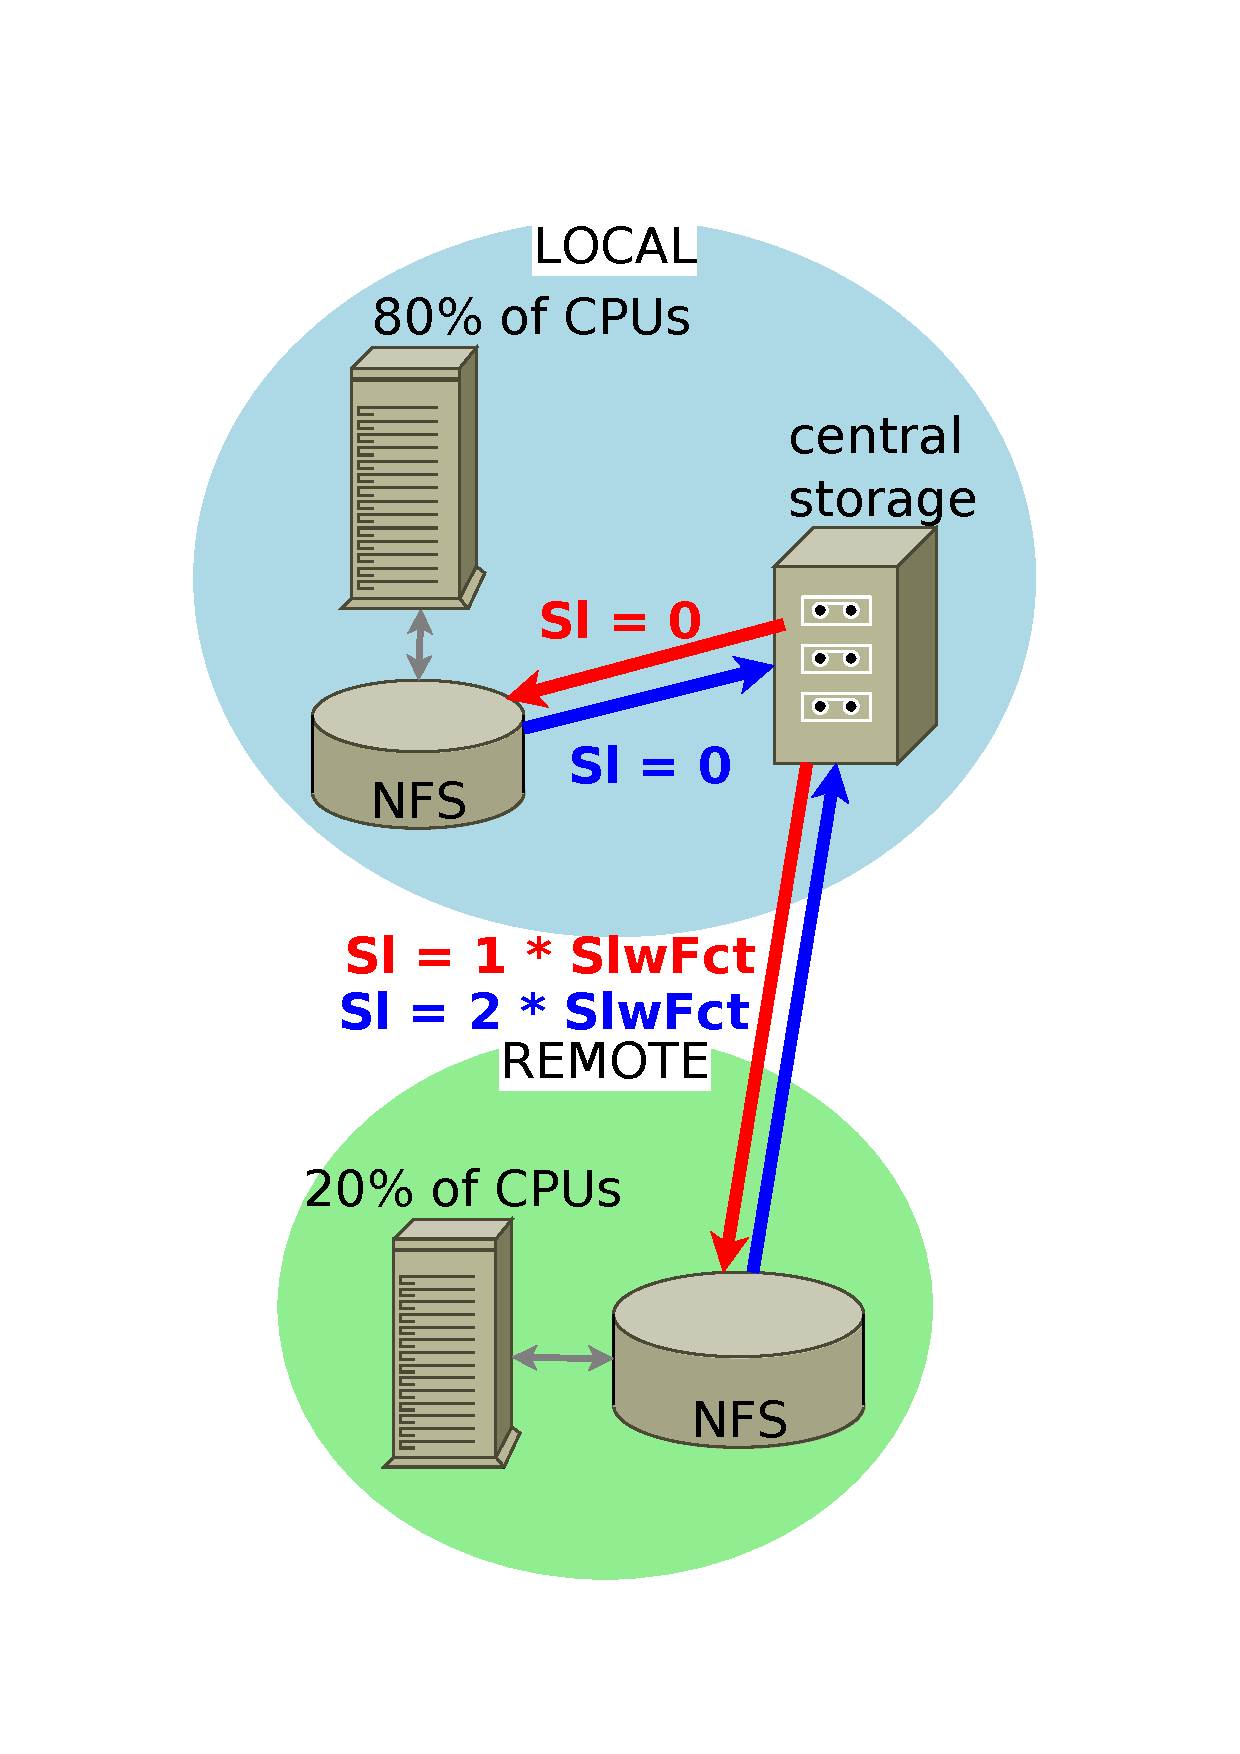
\includegraphics [width=1.2\textwidth]{pic/test_environment2.pdf}
			\end{center}
			\end{figure} 	 
\vspace{-1cm}
\begin{tiny}
\begin{center}
Constraints for storage capacity are omitted.
\end{center}
\end{tiny}
 	\end{columns} 	
\end{frame}

\begin{frame}\frametitle{Simulations based on log data: results.}
	%\vspace{-1cm}
	\begin{center}
    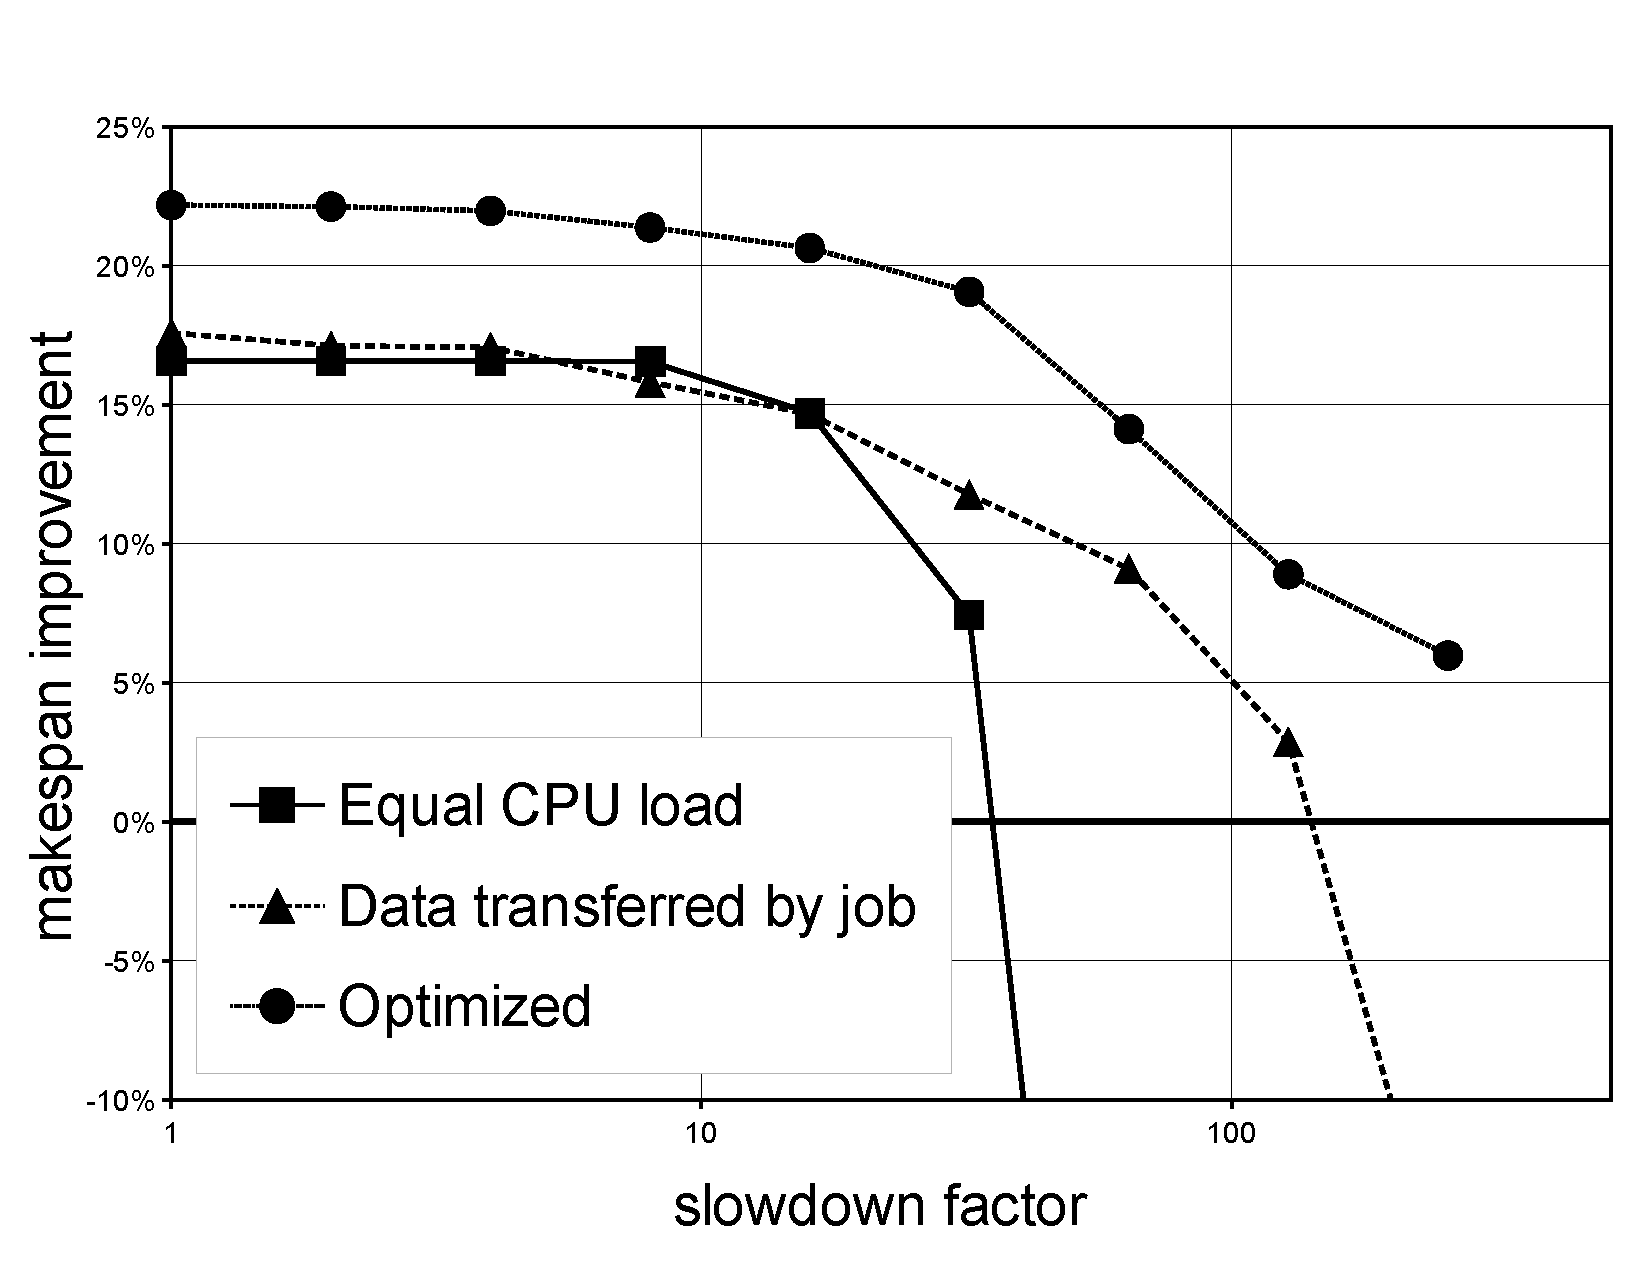
\includegraphics[trim =5mm 5mm 5mm 10mm ,clip,width=0.8\textwidth]{pic/makespan_vs_slowdown4.pdf}
	\end{center}
\end{frame}

 	
\begin{frame}\frametitle{Results of simulations}

\begin{footnotesize}
		\begin{itemize}
			\item In simulated environment, where a remote site has the same CPU number as a local site, but data transfer overhead is comparable to job duration: 
			\begin{itemize}
			\item Maintaining \textbf{equal CPU load} at local and remote sites increases the makespan more then twice; 
			\item Scheduling with \textbf{consideration of transfer overhead} can reduce makespan by 15\%.			\end{itemize}
			compared to \textbf{local only} processing.
			\item The simulations based on log files has shown that the proposed approach systematically provides a smaller makespan and adapts to the increase of transfer overheads better then the other simulated  heuristics.
			\item Proposed approach can provide \textbf{optimization} and \textbf{automatic adaptation} to fluctuating resources with no need for manual adjustment of work-flow at each site or tuning of heuristics.
		\end{itemize}		
\end{footnotesize}
\end{frame} 	

\section{Resource load planning}

\section{Enabling Caching}

\begin{frame}\frametitle{Enabling Caching}
\begin{block}{}
\vspace{-5mm}
    \begin{itemize}
        \item Performance of cache algorithms implemented with watermarking concept was simulated for a wide scope of cache size and low marks. 3 access patterns of 2 different experiments were used as input for simulations. 27 algorithms were tested in 90 simulation setups.        
    \end{itemize}
\end{block} 
\vspace{-2mm}
\begin{block}{Motivation}
    \begin{itemize}
        \item Cache of data-transfer tools.   
        \item Management of local data replicas. 
    \end{itemize}
   
\end{block}    


\begin{footnotesize}
\vspace{-2mm}
\begin{block}{Access patterns used for simulation}
\begin{itemize}
	\item[]\textbf{\textcolor{red}{STAR1:}} RCF@BNL, \textbf{Tier-0} for STAR experiment, Xrootd log, user analysis,  3 months period (June-August 2012).

	\item[]\textbf{\textcolor{green}{STAR2:}} RCF@BNL, \textbf{Tier-0} for STAR experiment, Xrootd log, user analysis, 7 months period (August 2012 - February  2013).

	\item[]\textbf{\textcolor{blue}{GOLIAS:}} FZU Prague, part of \textbf{Tier-2} of ATLAS. ATLAS and AUGER experiments, DPM log, user analysis + production,  3 months period (November 2012 - February  2013). AUGER makes less than  1\% of total requests.
\end{itemize}
\end{block}
\end{footnotesize}            
\end{frame}

\begin{frame}\frametitle{Selected caching algorithms}
\begin{footnotesize}
\begin{itemize}
\item \textbf{First-In-First-Out (FIFO)}: evicts files in the same order they entered the cache.
\item\textbf{Least-Recently-Used (LRU)}: evicts the set of files which were not used for the longest period of time.

\item \textbf{Least-Frequently-Used (LFU)}: evicts the set of files which were requested less times since they entered the cache.

\item \textbf{Most Size (MS)}: evicts the set of files which have the largest size.

\item \textbf{A}daptive \textbf{R}eplacement \textbf{C}ache (\textbf{ARC}). 2 lists: L1 - files with $access~count=1$, and L2 - files with $access~count>1$. LRU is applied to both list. The length of each list depends on $p = cache~hits~in~L1 / cache~hits~in~L2$.


\item \textbf{L}east \textbf{V}alue based on \textbf{C}aching \textbf{T}ime (\textbf{LVCT}).
Deletes files according to the value of the  Utility Function.
\begin{equation}
Utility Function = \frac{1}{Caching Time \times File Size}
\end{equation}   
where \textbf{Caching Time} of a file F is the sum of size of all files accessed after the last request for the file F.

\end{itemize}
\end{footnotesize}
\end{frame}

\begin{frame}\frametitle{What caching algorithm is the best? }
\vspace{-5mm}
  \begin{block}{Average improvement over FIFO}

	\begin{table}\begin{tabular}{|l|c|c|c|c|}
\hline
Algorithm & cache hits & cache data hits\\ \hline

MS & \textcolor{green}{116} \% & \textcolor{red}{-20} \% \\ \hline
LRU & 8 \% & 5 \% \\ \hline
LFU & -27 \% & -18 \% \\ \hline
ARC & 13\% & \textcolor{green}{11}\%\\ \hline
LVCT & \textcolor{green}{86} \%& 2 \%\\ \hline
\end{tabular}	
\end{table}
  \end{block}  
  
\begin{footnotesize}
\begin{block}{For studied access patterns}
\begin{itemize}
\item Regardless of the cache size, Tier-level and specificity of experiment the LVCT and ARC appear to be the most efficient  caching algorithms.
\item If the goal is to minimize makespan due to a transfer startup overhead the LVCT algorithm should be selected.
	\item If the goal is to minimize the network load the ARC algorithm is an option.
\end{itemize}
\end{block}
\end{footnotesize}  
\end{frame}


\begin{frame}\frametitle{Dependence of cache performance on low mark}
\vspace{-0.4cm}
\begin{tiny}	cache size / storage size = 0.1 ,high mark = 0.95 \end{tiny}
\begin{figure}
\vspace{-0.4cm}
	\begin{center}
		\centering
		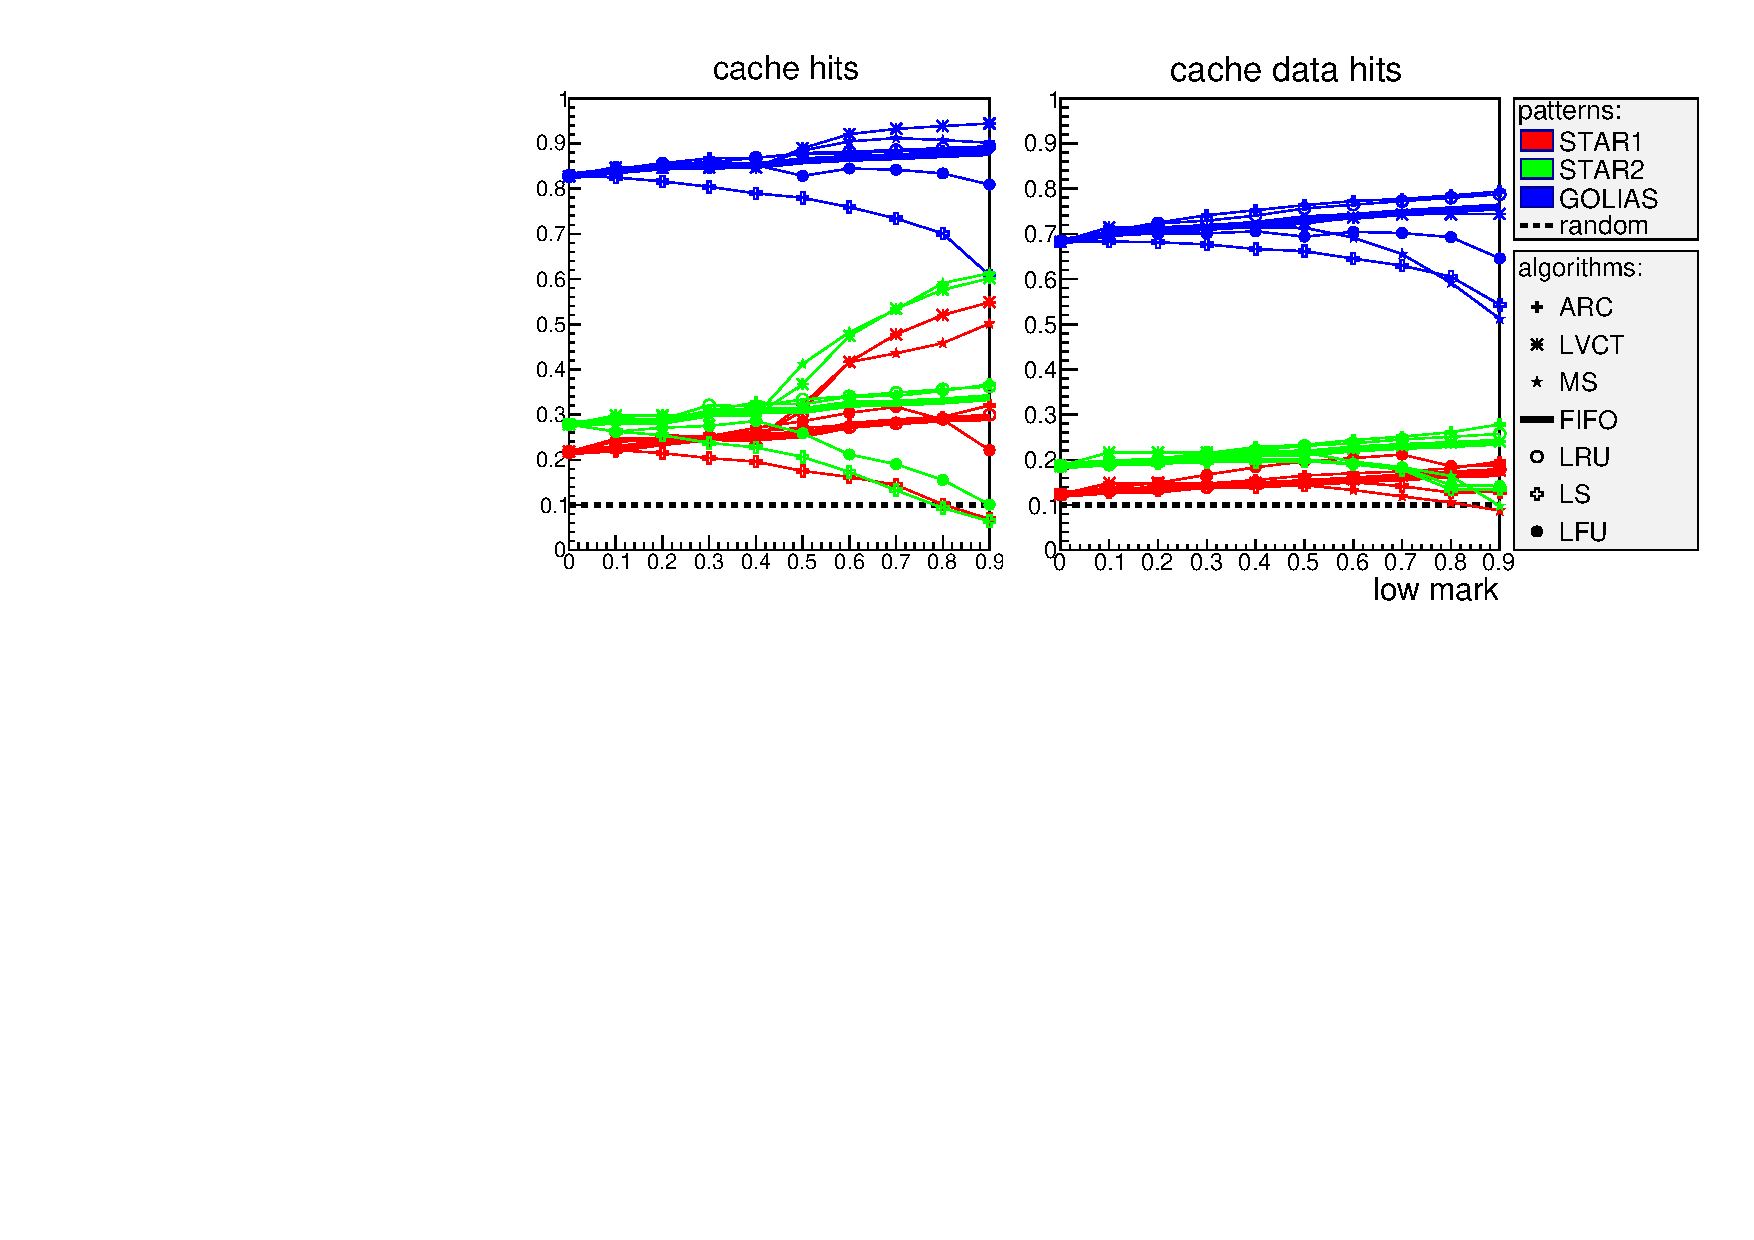
\includegraphics[width=\textwidth]{pic/low-basic_color.pdf}
		%\includegraphics[trim = 0mm 0mm 145mm 0mm,clip,height = 60mm]{pic/legendReady.pdf}
	\end{center}
\end{figure}	
\vspace{-0.5cm}
$\bullet $ Difference between Tier-2 and Tier-0 leads to distinct cache performance.\\
$\bullet $ With higher low mark the number of clean-ups increases as well as overall performance.\\


\end{frame}

\section{Conclusion and future plans}

\begin{frame}\frametitle{}

\end{frame}

\printbibliography

\end{document}
